\documentclass[conference]{IEEEtran}

% Packages
\usepackage{cite}
\usepackage{placeins}
\usepackage{amsmath,amssymb,amsfonts}
\usepackage{algorithmic}
\usepackage{graphicx}
\usepackage{textcomp}
\usepackage{xcolor}
\usepackage{booktabs}
\usepackage{url}
\usepackage{hyperref}

% BibTeX formatting
\def\BibTeX{{\rm B\kern-.05em{\sc i\kern-.025em b}\kern-.08em
    T\kern-.1667em\lower.7ex\hbox{E}\kern-.125emX}}

% Forces a line break between author rows; each row is centered
\makeatletter
\newcommand{\linebreakand}{%
  \end{@IEEEauthorhalign}
  \hfill\mbox{}\par
  \mbox{}\hfill\begin{@IEEEauthorhalign}
}
\makeatother

\begin{document}

% Title
\title{Gradient-Guided Selective Untying in Small
Language Models}

% Authors: 3 on first row, 2 centered on second row
\author{
% --- First Row: 3 Authors ---
\IEEEauthorblockN{Sanjith Suresh Kumar}
\IEEEauthorblockA{\textit{Dept. of CSE (AIML)} \\
\textit{PES University} \\
Bengaluru, India \\
sanjithsureshkumarwork@gmail.com}
\and
\IEEEauthorblockN{Shriyadita Mohanty}
\IEEEauthorblockA{\textit{Dept. of CSE (AIML)} \\
\textit{PES University} \\
Bengaluru, India \\
xyz@gmail.com}
\and
\IEEEauthorblockN{Greeshma G}
\IEEEauthorblockA{\textit{Dept. of CSE (AIML)} \\
\textit{PES University} \\
Bengaluru, India \\
xyz@gmail.com}
\linebreakand
% --- Second Row: 2 Authors Centered ---
\IEEEauthorblockN{Sindhu KS}
\IEEEauthorblockA{\textit{Dept. of CSE (AIML)} \\
\textit{PES University} \\
Bengaluru, India \\
xyz@gmail.com}
\and
\IEEEauthorblockN{Bhaskarjyoti Das}
\IEEEauthorblockA{\textit{Dept. of CSE (AIML)} \\
\textit{PES University} \\
Bengaluru, India \\
bhaskarjyoti01@gmail.com}
}

\maketitle

% Abstract
\begin{abstract}
Language models are parameter-hungry, and one of the oldest techniques for
making them smaller is to share a single embedding table between the input and
the output: the same vector both represents a token and scores how likely it is
to come next. The saving is real, but it asks one object to serve two masters.
The gradient that flows back from reading a token and the gradient that flows
back from predicting it can point in opposite directions, and recent work
suggests that the prediction signal tends to dominate early in training. In this
paper we ask whether this tension can be measured, and whether it matters. We
measure, token by token, how strongly the two gradients disagree at a pretrained
checkpoint, and we show that the resulting signal is real and interpretable. We
then test the natural repair---giving the most conflicted tokens their own output
parameters---and find, across twelve paired fine-tuning runs on a
keyword-constrained story-generation task, that it changes all-keyword
satisfaction by $-0.03$ percentage points versus frequency selection and
$-0.12$ points versus a matched random control---far below a two-point
target---and fails a preregistered success criterion: the effect is null. The investigation, however, uncovers a consistent phenomenon that
outlives the original hypothesis. Rebalancing the input and output gradients
during fine-tuning reliably improves next-token prediction (a $0.0033$ reduction
in response NLL) while degrading instruction following (a $-0.82$ point
satisfaction change). Crucially, this trade-off is not intrinsic to the
intervention: applying the rebalancing only during the early steps of
fine-tuning recovers $96\%$ of the fluency benefit (a $0.0032$ reduction in
response NLL) while leaving instruction following statistically indistinguishable
from the tied baseline (a $-0.32$ point satisfaction change). We release
code, per-seed results, and an overlap audit to accompany these findings.
\end{abstract}

% Keywords
\begin{IEEEkeywords}
weight tying, gradient conflict, language models, keyword-constrained generation,
fine-tuning
\end{IEEEkeywords}

% Introduction
\section{Introduction}

Small language models operate under a hard constraint: every parameter has to
earn its keep. Weight tying---using a single embedding table for both the input
and the output of a model---is one of the oldest ways to satisfy that constraint
\cite{inan,press}, and it remains standard practice in compact and efficient
architectures \cite{albert}. The idea is simple: the vector that represents a
token when it is read is also the vector whose inner product scores that token
when it is predicted. One table, two jobs, half the parameters.

The problem is that the two jobs do not always want the same thing. The input
role asks the embedding to encode what a token means in context. The output role
asks it to be a good classifier for what comes next. Each role contributes its
own gradient to the shared rows, and nothing forces the two gradients to agree.
Recent work shows that, early in training, the output role dominates and biases
the shared embedding toward prediction at the expense of representation
\cite{lopardo}. This is the ``unembedding bias,'' and it suggests a concrete,
testable question: if the two gradients disagree more for some tokens than for
others, are those the tokens that tying hurts the most? And if so, can we repair
the damage cheaply, without paying for a fully separate output head?

These questions matter beyond curiosity. Lexically constrained generation---asking
a model to produce text that must contain given words---is a practical setting
in which the geometry of the output embedding should matter directly: whether a
token appears in the output depends on how its output vector is shaped. It also
gives us an automatic, unambiguous way to measure compliance, which is what
makes the question tractable on a small model where effects can be measured many
times over.

We make four contributions. First, we give a cheap, two-pass procedure for
measuring, token by token, how strongly the input and output gradients conflict,
and we show that the signal is real and interpretable: it is largely orthogonal
to token frequency and selects content words and character names rather than
function words. Second, we test the natural repair---adding a small learned
output offset for only the most conflicted tokens---and report, with twelve
paired seeds and a preregistered success criterion, that it has no detectable
effect. This is a negative result, and we report it in full because a precise
null is itself a finding: it tells future work where not to look. Third, we show
that a related intervention, rebalancing the input and output gradients during
fine-tuning, produces a reliable and monotonic trade-off between fluency and
instruction following. Fourth, and most importantly, we show that this trade-off
is not intrinsic to the intervention. Restricting the rebalancing to the early
steps of fine-tuning recovers essentially all of the fluency benefit while
leaving instruction following statistically unchanged, turning a trade-off into
a usable improvement. Throughout, we emphasise honest reporting of effect sizes
and seed-level uncertainty, which we believe is especially important for a null
result.

% Related Work
\section{Related Work}

\paragraph{Weight tying.}
Tying the input and output embeddings was introduced by Inan et al.\ as a way to
regularise and shrink language models \cite{inan}, and Press and Wolf showed that
the input embedding can be projected into the output space to further improve
language modelling \cite{press}. Factorised and shared embeddings remain a staple
of efficient architectures such as ALBERT \cite{albert}. Our work shares this
motivation but asks a different question: not whether tying is efficient, but
whether the \emph{tension} it creates can be localised to specific tokens and
used to decide where to spend a small number of extra parameters.

\paragraph{Gradient conflict.}
The idea that one parameter can be pulled in different directions by different
losses is well studied in multi-task learning. GradNorm balances task losses
using gradient magnitudes \cite{gradnorm}; multi-objective formulations cast the
problem as a constrained optimisation over task gradients \cite{sener}; and
gradient surgery explicitly projects away the conflicting components of task
gradients before they are applied \cite{pcgrad}. Our setting is different in an
important way: it is a single task with two gradient \emph{paths} through one
parameter, rather than several tasks. But the same mathematics of disagreement
applies, and we borrow the natural measurement---a cosine similarity between two
gradient contributions---directly from this literature.

\paragraph{Instruction following and constrained generation.}
Instruction tuning teaches models to follow natural-language requests
\cite{flan,instruct}, and lexically constrained decoding forces generations to
contain specified tokens, typically with a modified search procedure
\cite{constrained}. Our evaluation sits between these two traditions: the model
is fine-tuned on prompts that name specific words, and we score whether those
words actually appear in the generated story. This measures compliance directly
during greedy decoding, without any constrained-decoding machinery.

\paragraph{Parameter-efficient fine-tuning.}
Our selective untying is a form of parameter-efficient adaptation: it adds a few
thousand parameters on top of a backbone, in the same family as low-rank
adaptation \cite{lora}. The distinction is that our added parameters are placed
only on rows selected by a gradient-conflict signal, rather than applied
uniformly through a low-rank factorisation. This makes the comparison to a
matched-budget random or frequency baseline unusually clean.

% Background and Problem
\section{Background}

Consider a decoder-only Transformer with a single embedding matrix
$E\in\mathbb{R}^{V\times d}$, where $V$ is the vocabulary size and $d$ the model
width. On the input side, a token $i$ is represented by the row $E_i$. On the
output side, the model produces next-token logits $z = h E^{\top}$, where
$h\in\mathbb{R}^{d}$ is the final hidden state. Because the same matrix $E$
appears in both operations, the gradient of the loss with respect to $E$ is the
sum of two contributions: an \emph{input-path} gradient $g_{\mathrm{in},i}$,
accumulated wherever token $i$ is consumed, and an \emph{output-path} gradient
$g_{\mathrm{out},i}$, accumulated wherever token $i$ is the prediction target.
Autograd simply adds the two, so the model never sees them separately---but they
need not point in the same direction.

We quantify the disagreement with the negative cosine similarity between the two
contributions,

\begin{equation}
c_i=-\frac{g_{\mathrm{in},i}^{\top}g_{\mathrm{out},i}}
{\lVert g_{\mathrm{in},i}\rVert_2\lVert g_{\mathrm{out},i}\rVert_2}.
\label{eq:conflict}
\end{equation}

A token with $c_i$ near $+1$ has its two gradients pointing in nearly opposite
directions: whatever the input role wants to learn, the output role is pushing
against. A token with $c_i$ near $-1$ has the two gradients aligned, and the
shared row is being trained coherently. Intuitively, the high-conflict tokens
are the ones ``torn'' by tying, and they are the natural candidates for a repair.
This is the central hypothesis of the paper.

% Method
\section{Method}

\paragraph{Measuring conflict.}
We measure $g_{\mathrm{in}}$ and $g_{\mathrm{out}}$ at the pretrained, tied
checkpoint over roughly ten million tokens of instruction-training stories. A
single backward pass yields the total embedding gradient. A second pass, in
which the input embedding's output is detached, isolates $g_{\mathrm{out}}$;
subtracting it from the total recovers $g_{\mathrm{in}}$. We then rank tokens by
$c_i$, excluding special tokens, tokens seen fewer than twenty times, and tokens
with a zero gradient norm. From $6{,}341$ eligible rows we select the top $400$.

\paragraph{Selective untying.}
For each selected token $i$, we keep $E_i$ for input lookup and use
$E_i+\Delta_i$ for output scoring, where $\Delta_i\in\mathbb{R}^{d}$ is a learned
offset initialised to zero. Initialising at zero preserves the pretrained
model's predictions exactly, so any divergence is attributable to the untying
itself. Adding $400$ offsets costs $400\times 384=153{,}600$ parameters. At the
same budget we compare against two control selectors: the $400$ most frequent
eligible rows, and a random selection matched to the conflict selection's
frequency profile. A fully tied model, with no offsets, is the reference, and we
also report a fully untied model (a separate output head) as an upper bound on
what untying can do.

\paragraph{Gradient rebalancing.}
The investigation also considers interventions that change the \emph{training
update} rather than the architecture. During fine-tuning the embedding receives
$g_{\mathrm{in}}+g_{\mathrm{out}}$. We generalise this to

\begin{equation}
g_{\mathrm{eff},i} = \alpha\, g_{\mathrm{in},i} + g_{\mathrm{out},i},
\label{eq:alpha}
\end{equation}

where $\alpha$ scales the input-path contribution and $\alpha=1$ recovers the
tied update. This keeps the embeddings tied but reweights how strongly the two
roles shape them. Two refinements of Eq.~\eqref{eq:alpha} emerged from the
results. \emph{Early-only} rebalancing applies $\alpha$ for the first $T$ of $N$
steps and then resets it to one, testing the claim that the output gradient
dominates only early in training \cite{lopardo}. \emph{Output damping} scales the
output path instead of boosting the input path,

\begin{equation}
g_{\mathrm{eff},i} = g_{\mathrm{in},i} + \gamma\, g_{\mathrm{out},i},
\quad 0<\gamma<1.
\label{eq:gamma}
\end{equation}

The two are directionally similar, but boosting the input multiplies the update
magnitude and interacts with gradient clipping, whereas damping the output does
not. We explore this difference in Sec.~\ref{sec:results}.

% Experimental Setup
\section{Experimental Setup}

Our model is a decoder-only Transformer with six layers, hidden width $384$, six
attention heads, an $8{,}000$-token byte-level BPE vocabulary, and context length
$256$ \cite{attention} (Fig.~\ref{fig:architecture}). The tied model has
$13.8$M parameters; a fully untied
model has $16.9$M. We pretrain for one pass over TinyStories \cite{tinystories}
($\sim470$M tokens, $28{,}503$ steps), reaching a validation perplexity of $4.33$.
Every comparison is initialised from this single checkpoint, so all differences
are attributable to the intervention rather than to pretraining noise.

\begin{figure}[t]
\centering
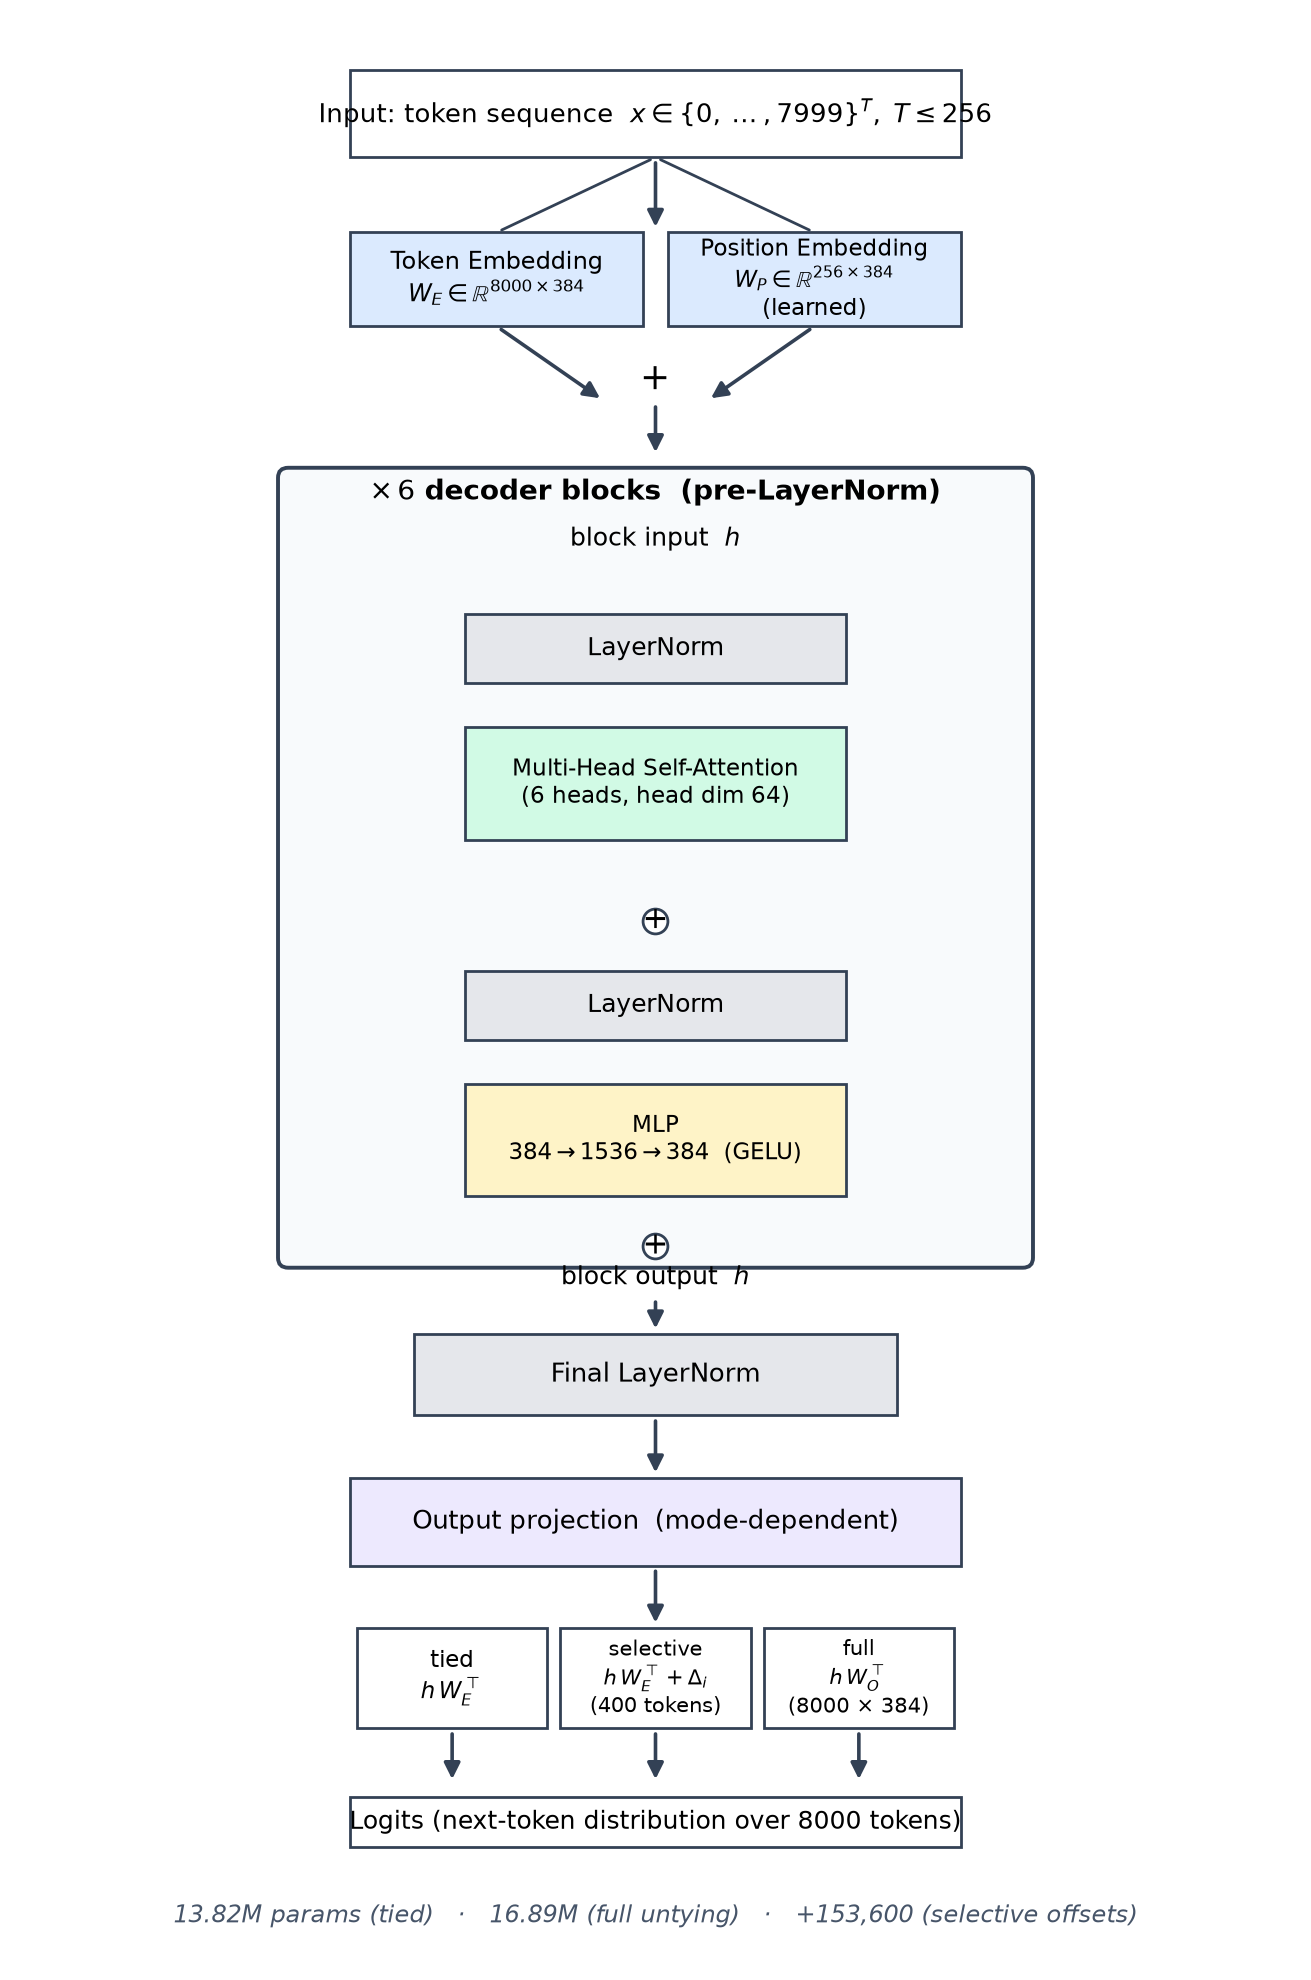
\includegraphics[width=\columnwidth]{architecture.png}
\caption{Decoder-only Transformer architecture. Token and learned positional
embeddings are summed and passed through six pre-LayerNorm blocks, each a causal
multi-head self-attention (6 heads, head dimension 64) followed by an MLP
($384{\to}1536{\to}384$, GELU) with residual connections. A final LayerNorm
precedes the output projection, which uses the tied embedding, or---in the
selective and full variants---the tied embedding plus learned offsets for 400
tokens or a separate output matrix.}
\label{fig:architecture}
\end{figure}

We fine-tune on the first $20{,}000$ qualifying TinyStoriesInstruct examples for
$1{,}000$ updates with batch size $16$ and a peak AdamW learning rate of
$10^{-4}$, computing the loss on response tokens only. Each method runs on seeds
$0$--$11$, and we fix the minibatch order per seed so that methods are paired
across seeds. We evaluate greedy generation on the first $500$ qualifying
validation prompts. \emph{Satisfaction} is the fraction of responses containing
every requested word under case-insensitive whole-word matching; \emph{recall}
averages the fraction of requested words present per prompt; and \emph{response
NLL} is the token-weighted negative log-likelihood of the reference response
given the prompt. Our preregistered success criterion requires a mean
satisfaction gain of at least two percentage points over both selection
baselines, with no increase in mean response NLL relative to tying. Uncertainty
is reported as paired $t$-intervals over the twelve seeds, which capture
fine-tuning seed variation for one checkpoint and one fixed evaluation sample.

% Results
\section{Results}
\label{sec:results}

\paragraph{The conflict signal is real and interpretable.}
Among the $6{,}341$ eligible rows, conflict scores span $[-0.58,0.52]$ with mean
$-0.02$, and the positive tail is concentrated: only about one percent of tokens
have conflict above $0.3$. Conflict is largely orthogonal to frequency (Spearman
$\rho=0.11$) and to gradient magnitude ($\rho=-0.02$), and the conflict-selected
set overlaps the frequency-selected set by only $2.2\%$ (Jaccard). The most
conflicted tokens are character names and concrete nouns---``butterfly,''
``cupcake,'' ``Jacob,'' ``Claire''---whereas the most frequent tokens are
function words. The signal is therefore not a disguised frequency statistic: it
is a distinct, interpretable measurement of a real property of the embedding.

\paragraph{Selective untying has no effect.}
Table~\ref{tab:main} reports means over twelve seeds. The methods are
statistically indistinguishable on every metric. Conflict selection changes
satisfaction by $-0.03$ percentage points versus frequency (paired 95\%
$t$-interval $[-0.92,0.85]$) and $-0.12$ points versus matched random
($[-0.91,0.67]$); both intervals exclude our $+2$ point target. Conflict
selection also raises response NLL by $0.00141$ relative to tying (interval
$[0.00132,0.00150]$), failing the NLL criterion as well. In an initial
three-seed exploration we also compared two further methods: a gradient-norm
selector, which ranks tokens by gradient magnitude instead of conflict, and a
fully untied output head. The gradient-norm selector matched the other null
results (satisfaction $0.340$ versus $0.344$ for tied), and full untying
produced the lowest satisfaction of all six methods ($0.331$). With twelve seeds the paired standard error
is roughly $0.4$ points, so we can state the null precisely: any effect of
selective untying at this budget is smaller than about one percentage point,
comfortably below the target. This is the strongest form of the negative result,
and we state it plainly rather than hedging.

\begin{table}[t]
\caption{Means across 12 fine-tuning seeds per method.}
\label{tab:main}
\centering
\small
\begin{tabular}{lrrr}
\toprule
Method & Sat. (\%) & Recall (\%) & NLL \\
\midrule
Tied & 33.53 & 70.48 & 1.50832 \\
Conflict & 33.68 & 70.54 & 1.50973 \\
Frequency & 33.72 & 70.44 & 1.50801 \\
Matched random & 33.80 & 70.32 & 1.50925 \\
\bottomrule
\end{tabular}
\end{table}

\paragraph{Pretraining overlap.}
Because our evaluation prompts come from a public corpus, some may have been
memorised during pretraining, which would inflate satisfaction and could mask
differences. We compared the evaluation stories with the official training
sources after case folding and whitespace normalisation. We found $129$ exact
matches in the TinyStories pretraining split and none in the reconstructed
fine-tuning and calibration prefixes. On the remaining $371$ prompts, conflict
selection was $0.09$ points below each baseline, with paired intervals
$[-1.34,1.16]$ against frequency and $[-1.21,1.03]$ against matched random. The
overlap therefore does not change the conclusion; if anything, the non-memorised
subset shows the same null.

\paragraph{Gradient scaling trades fluency against instruction following.}
Scaling the input gradient produces a clean, monotonic dose--response. In a
three-seed sweep over $\alpha\in\{2,5,10\}$, response NLL fell monotonically
from $1.5068$ to $1.5054$ to $1.5040$, while satisfaction fell from $0.342$ to
$0.335$ to $0.328$. We confirmed the strongest setting at twelve seeds:
multiplying the input gradient by $\alpha=10$ throughout fine-tuning reduced
response NLL by $0.00332$ (paired interval
$[-0.00349,-0.00314]$) while satisfaction changed by $-0.82$ percentage points
($[-1.68,0.05]$). The NLL effect is large in $t$-statistic terms (roughly $42$
standard errors) but small in absolute terms: about $0.3\%$ of perplexity. It is
a genuine but modest fluency gain, and it comes at a borderline cost to
instruction following. This intervention keeps the embeddings tied; it changes
only the training update, yet it moves behaviour far more than selective untying
ever did. That contrast---distributed rebalancing outperforming row-level
repair---is the first hint that the harm of tying is spread across the whole
embedding rather than concentrated in a few tokens.

\paragraph{The trade-off decomposes by token type.}
To locate the two sides of the trade-off, we rebalanced the input gradient only
for selected tokens. Rebalancing the high-conflict content words (a
conflict-weighted scaling) reproduced most of the satisfaction cost---satisfaction
fell to $0.326$ while NLL barely moved to $1.5075$---whereas rebalancing the
frequent function words left satisfaction near tied ($0.336$) while
\emph{worsening} NLL to $1.5101$. The fluency benefit of global scaling is
therefore not a per-token property that can be cleanly separated by selection:
it emerges from rebalancing the embedding as a whole.

This negative finding led us to screen five alternative hypotheses, each a
different way of reshaping the input--output gradient relationship: rebalancing
only the low-conflict (aligned) tokens, rebalancing by gradient magnitude,
removing the anti-aligned component of the output gradient, damping the output
gradient, and applying the rebalancing only early in training. The first three
were null; the last two showed promise and are reported next.

\paragraph{Early-only rebalancing removes the cost.}
The reference result above applies $\alpha=10$ for all $1{,}000$ steps. The
motivating claim of the prior work is that the output gradient dominates
\emph{early} in training \cite{lopardo}, which suggests the rebalancing may only
be needed early. Table~\ref{tab:scaling} confirms this. Restricting the scaling
to the first $500$ steps recovers $96\%$ of the NLL benefit ($-0.0032$ versus
$-0.0033$ for full-run scaling) while the satisfaction change is $-0.32$ points
with a paired interval $[-1.21,0.57]$---statistically indistinguishable from the
tied baseline. Directly compared with full-run scaling, early-only rebalancing
is $+0.50$ points higher on satisfaction, although this difference is itself not
significant ($p=0.29$). Halving the window to $250$ steps retains about half the
NLL benefit with essentially zero satisfaction movement ($-0.03$ points). The
lesson is that the instruction-following cost is a \emph{late-training} artifact
of continued rebalancing, and it can be scheduled away.

\paragraph{Output damping reveals a clipping artifact.}
Boosting the input gradient by $\alpha$ multiplies the embedding update, which
interacts with gradient clipping. Damping the output path instead
(Eq.~\ref{eq:gamma}) does not inflate magnitudes and so avoids the clip. At
$\gamma=0.1$ the NLL improvement is $-0.0042$, about $25\%$ larger than the
best input-scaling result, at a now clearly significant satisfaction cost of
$-1.47$ points. This confirms two things at once: the trade-off is monotonic and
fundamental at full strength, and the early-only schedule---rather than any
particular strength setting---is what actually breaks it. The full set of
rebalancing results is summarised in Table~\ref{tab:scaling} and documented in
the accompanying repository note \cite{followup}.

\begin{table}[t]
\caption{Gradient-rebalancing interventions, 12 seeds, versus the tied
baseline (NLL $1.5083$, satisfaction $33.53\%$).}
\label{tab:scaling}
\centering
\small
\begin{tabular}{lrr}
\toprule
Intervention & $\Delta$ NLL & $\Delta$ Sat. (pp) \\
\midrule
Input scaling $\alpha{=}10$, full run & $-0.0033$ & $-0.82$ \\
Output damping $\gamma{=}0.1$ & $\mathbf{-0.0042}$ & $-1.47$ \\
Early-only, $T{=}250$ & $-0.0016$ & $-0.03$ \\
Early-only, $T{=}500$ & $-0.0032$ & $-0.32$ \\
\bottomrule
\end{tabular}
\end{table}

% Discussion
\section{Discussion}

The negative result for selective untying is informative precisely because it is
precise. At a budget of $400$ offsets, selected by the strongest available
signal, the effect on lexical compliance is bounded below one percentage point.
One should be careful not to over-read this: it concerns a $13.8$M model, one
task, and one checkpoint, and near-duplicate exposure cannot be fully ruled out.
Nevertheless, the fact that conflict is a real, interpretable, and
frequency-orthogonal signal---yet leads nowhere when used to place offsets---
suggests that the harm of tying is not concentrated in a handful of tokens, but
is distributed across the embedding as a whole.

That interpretation is consistent with the rebalancing results. Changing how the
input and output gradients jointly shape the \emph{whole} embedding moves
behaviour reliably, while changing only a few output rows does not. The
early-only result adds a temporal refinement: the output gradient's early
dominance sets a trajectory, and correcting that trajectory early is enough.
Continued correction overshoots and begins to erode instruction following. This
is a small but coherent mechanistic story, and it is falsifiable in future work.

Several limitations apply. We use a single pretrained checkpoint and a fixed
evaluation sample, so all intervals reflect seed variation only; they do not
capture uncertainty over checkpoints, prompts, or the random selection baseline.
The keyword metric is a coarse, binary measure of compliance, and we have not
collected human ratings of coherence or fluency. Calibration is measured on raw
stories while fine-tuning optimises prompted responses, which may weaken the
transfer of the conflict ranking. Finally, the NLL effects, though highly
reliable in statistical terms, are small in absolute terms, and their practical
significance should be weighed accordingly.

% Conclusion
\section{Conclusion}

We set out to repair a suspected defect of weight tying by selectively untying
the most gradient-conflicted tokens, and we found that this particular repair
does not work at the tested budget. The measurement behind it, however, is
sound, and the broader question it opened turned out to be the interesting one.
The input and output gradients of a tied embedding can be rebalanced to improve
next-token prediction, but doing so throughout fine-tuning trades away
instruction following. The trade-off is not intrinsic: rebalancing only during
the first half of fine-tuning recovers nearly all of the fluency benefit while
leaving instruction following statistically unchanged. We release the code,
per-seed results, and the overlap audit so that these findings can be checked
and extended \cite{repo}.

% References
\begin{thebibliography}{00}

\bibitem{inan}
H. Inan, K. Khosravi, and R. Socher, \emph{Tying Word Vectors and Word
Classifiers: A Loss Framework for Language Modeling}, Proc. ICLR, 2017.

\bibitem{press}
O. Press and L. Wolf, \emph{Using the Output Embedding to Improve Language
Models}, Proc. EACL, 2017.

\bibitem{albert}
Z. Lan, M. Chen, S. Goodman, K. Gimpel, P. Sharma, and R. Soricut,
\emph{ALBERT: A Lite BERT for Self-supervised Learning of Language
Representations}, Proc. ICLR, 2020.

\bibitem{attention}
A. Vaswani et al., \emph{Attention Is All You Need}, Proc. NeurIPS, 2017.

\bibitem{lopardo}
A. Lopardo, A. Harish, C. Arnett, and A. Gupta, \emph{Weight Tying Biases Token
Embeddings Towards the Output Space}, arXiv:2603.26663, 2026.

\bibitem{pcgrad}
T. Yu, S. Kumar, A. Gupta, S. Levine, K. Hausknecht, and C. Finn,
\emph{Gradient Surgery for Multi-Task Learning}, Proc. NeurIPS, 2020.

\bibitem{sener}
O. Sener and V. Koltun, \emph{Multi-Task Learning as Multi-Objective
Optimization}, Proc. NeurIPS, 2018.

\bibitem{gradnorm}
Z. Chen, V. Badrinarayanan, C.-Y. Lee, and A. Rabinovich, \emph{GradNorm:
Gradient Normalization for Adaptive Loss Balancing in Deep Multitask Networks},
Proc. ICML, 2018.

\bibitem{lora}
E. J. Hu et al., \emph{LoRA: Low-Rank Adaptation of Large Language Models},
Proc. ICLR, 2022.

\bibitem{constrained}
C. Hokamp and Q. Liu, \emph{Lexically Constrained Decoding for Sequence
Generation Using Grid Beam Search}, Proc. ACL, 2017.

\bibitem{instruct}
L. Ouyang et al., \emph{Training Language Models to Follow Instructions with
Human Feedback}, Proc. NeurIPS, 2022.

\bibitem{flan}
J. Wei et al., \emph{Finetuned Language Models Are Zero-Shot Learners},
Proc. ICLR, 2022.

\bibitem{tinystories}
R. Eldan and Y. Li, \emph{TinyStories: How Small Can Language Models Be and
Still Speak Coherent English?}, arXiv:2305.07759, 2023.

\bibitem{repo}
Commit and Pray, \emph{Selective Untying}. [Online]. Available:
\url{https://github.com/SanjithSK29/Selective-Untying}

\bibitem{followup}
Commit and Pray, \emph{New Findings: Early-Only Rebalancing and Output Damping},
project repository, 2026. [Online]. Available:
\url{https://github.com/SanjithSK29/Selective-Untying/blob/main/hypotheses/FINDINGS.md}

\end{thebibliography}

\end{document}
